\documentclass[12pt]{article}

\usepackage{pablo}
\usepackage[a5paper,margin=1cm]{geometry}
\usepackage{multicol}
\usepackage{tkz-tab}
\pagestyle{empty}

\begin{document}

\begin{center}
  \textsc{Devoir commun de mathématiques --- Sujet B}
\end{center}

\begin{exercice}~

  \subsubsection*{Partie A : Calculs algébriques}
  \emph{Soit $f$ la fonction définie sur $\mathbb{R}$ par $f(x)=-x^2+8x$.}
  \begin{enumerate}
    \item
      \begin{multicols}{2}
      \begin{enumerate}
        \item \emph{Calculer $f\left(\frac{1}{2}\right)$.}

          \begin{align*}
            f\left(\frac{1}{2}\right) &= -\left(\frac{1}{2}\right)^2+8\times\frac{1}{2}\\
                                      &= -\left(\frac{1^2}{2^2}\right)+\frac{8}{2}\\
                                      &= -\frac{1}{4}+\frac{8\times2}{2\times2}\\
                                      &= -\frac{1}{4}+\frac{16}{4}\\
                                      &= \frac{15}{4}\\
          \end{align*}

          \columnbreak

        \item \emph{Remplir le tableau de valeurs et tracer la courbe.}
            \begin{multicols}{2}
                \begin{tabular}{|c|c|}
                  \hline
                  $x$ & $f(x)$ \\
                  \hline
                  -0.5 & -4.25 \\
                  \hline
                  0 & 0 \\
                  \hline
                  0.5 & 3,75 \\
                  \hline
                  1 & 7 \\
                  \hline
                  1.5 & 9,75 \\
                  \hline
                  2 & 12 \\
                  \hline
                  2.5 & 13,75 \\
                  \hline
                  3 & 15 \\
                  \hline
                  3.5 & 15,75 \\
                  \hline
                  4 & 16 \\
                  \hline
                \end{tabular}

                \begin{tabular}{|c|c|}
                  \hline
                  $x$ & $f(x)$ \\
                  \hline
                  4.5 & 15,75 \\
                  \hline
                  5 & 15 \\
                  \hline
                  5.5 & 13,75 \\
                  \hline
                  6 & 12 \\
                  \hline
                  6.5 & 9,75 \\
                  \hline
                  7 & 7 \\
                  \hline
                  7.5 & 3,75 \\
                  \hline
                  8 & 0 \\
                  \hline
                  8.5 & -4,25 \\
                  \hline
                  &\\
                  \hline
                \end{tabular}
            \end{multicols}
      \end{enumerate}
            \end{multicols}

            \begin{center}
            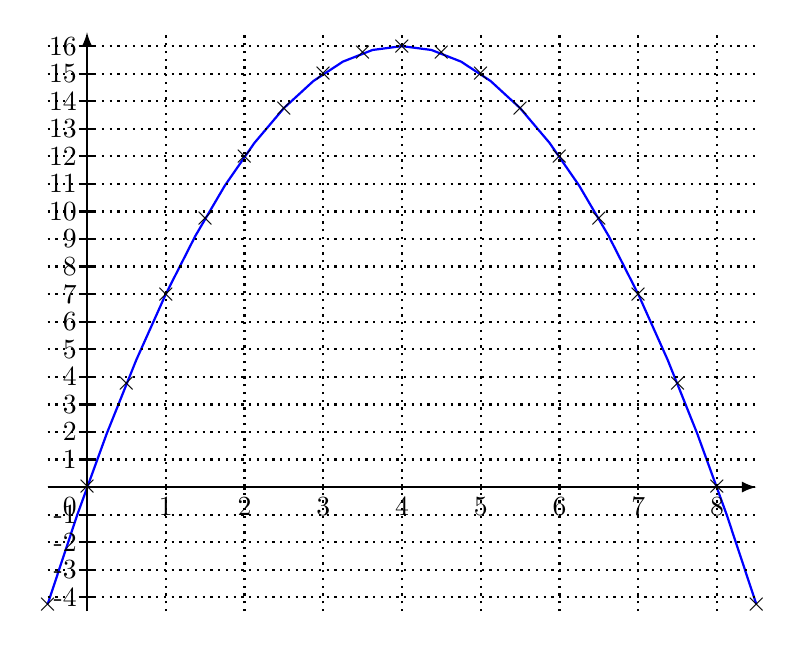
\begin{tikzpicture}[thick,xscale=1,yscale=0.35]
              \draw[color=blue,domain=-0.5:8.5] plot (\x,{-\x*\x+8*\x});
              \foreach \x in {-0.5,0,...,8.5}{
                \draw (\x, {-\x*\x+8*\x}) node{$\times$};
              }
              \foreach \x in {0,...,8} {
                \ifthenelse{\equal{\x}{0}}
                {}
                {
                  \draw (\x,-0.1) -- (\x,0.1);
                  \draw (\x,0) node[below]{\x};
                }
              }
              \foreach \y in {-4,...,16} {
                \ifthenelse{\equal{\y}{0}}
                {}
                {
                  \draw (-0.1,\y) -- (0.1,\y);
                  \draw (0,\y) node[left]{\y};
                }
              }
              \draw (0,0) node[below left]{0};
              \draw[-latex] (-.5,0) -- (8.5,0);
              \draw[-latex] (0,-4.5) -- (0,16.5);
              \draw[dotted] (-.5,-4.5) grid (8.5,16.5);
            \end{tikzpicture}
          \end{center}
    \item \emph{Factoriser $f$.}
          \begin{align*}
            f\left(x\right) &= -\left(x^2+8x\right)\\
                            &= x\left(-x+8\right)
          \end{align*}
        \item \emph{Montrer que pour tout $x\in\mathbb{R}$, on a $f(x)=(1-x)(x-7)+7$.} On développe le membre de droite.
          \begin{align*}
            (1-x)(x-7)+7 &= x -7-x(x-7)+7\\
                         &= x-7-x^2+7x+7\\
                         &= -x^2+8x\\
                         &= f(x)
          \end{align*}
        \item \emph{Montrer que pour tout $x\in\mathbb{R}$, on a $f(x)=-(x-4)^2+16$.} On développe le membre de droite.
          \begin{align*}
            -(x-4)^2+16 &= -\left(x^2-2\times4x+4^2\right)+16\\
                       &= -x^2+8x-16+16\\
                       &= -x^2+8x\\
                       &= f(x)
          \end{align*}
        \item~
          \begin{enumerate}
            \item \emph{Résoudre $f(x)=0$.} On utilise la forme factorisée.
          \begin{align*}
            && f(x) &= 0\\
            &\iff& x(-x+8)&=0\\
            &\iff& x=0 &\text{ ou } -x+8=0\\
            &\iff& x=0 &\text{ ou } x=8
          \end{align*}
        \item \emph{Résoudre $f(x)\geq7$.} On utilise la forme $f(x)=(1-x)(x-7)+7$.
          \begin{align*}
            && f(x) &\geq 7\\
            &\iff& (1-x)(x-7)+7 &\geq7\\
            &\iff& (1-x)(x-7) &\geq0
          \end{align*}
          Nous obtenons une inéquation produit, que l'on résout en utilisant un tableau de signes.
  \begin{center}
  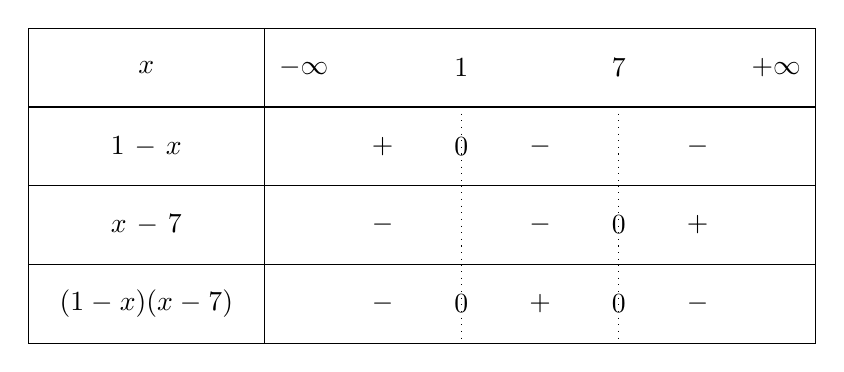
\begin{tikzpicture}
    \tkzTabInit[lgt=3,espcl=2]{$x$ /1, $1-x$ /1, $x-7$ /1, $(1-x)(x-7)$/1 }%
    {$-\infty$ ,$1$ , $7$, $+\infty$}%
    \tkzTabLine{,+,z,-,t,-}
    \tkzTabLine{,-,t,-,z,+}
    \tkzTabLine{,-,z,+,z,-}
  \end{tikzpicture}
\end{center}
La solution se lit sur la dernière ligne : $(1-x)(x-7)\geq0$ pour $x\in\left[1;7\right]$, donc $f(x)\geq7$ pour $x\in\left[1;7\right]$.
\item
  \begin{multicols}{2}
    La fonction $f$ est un trinôme du second degré, et le facteur de $x^2$
    est négatif, donc la fonction est croissante puis décroissante.
    L'abscisse de l'extrémum est $-\frac{b}{2a}$, soit
    $-\frac{8}{2\times-1}=4$. L'ordonnée de cet extrémum est $f(4)=16$.

    \columnbreak

  \begin{center}
    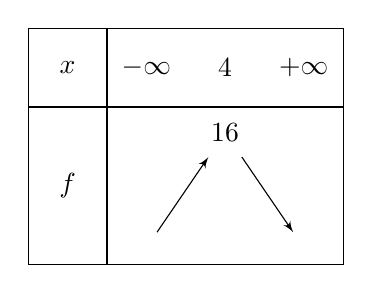
\begin{tikzpicture}
      \tkzTabInit[lgt=1,espcl=1]
      {$x$ /1,
      $f$ /2}
      {$-\infty$,$4$,$+\infty$}%
      \tkzTabVar{-/, +/16, -/}
    \end{tikzpicture}
  \end{center}
\end{multicols}
          \end{enumerate}
  \end{enumerate}

  \subsubsection*{Partie B : Modélisation}
  \begin{enumerate}
    \item $x$ est la longueur $CE$, $E$ appartenant au segment $[CD]$. Donc
      $x\in\left[0;8\right]$.
    \item Le segment $[ED]$ a pour longueur $8-x$, donc l'aire $A(x)$ de $EFGD$ vaut $A(x)=x(8-x)$.
    \item On reconnait dans $A(x)$ la forme factorisée de $f$ (étudiée dans
      la partie A). Donc résoudre $A(x)\geq7$ revient à résoudre $f(x)\geq7$.
      Ceci a été résolu dans la partie précédente, et on trouve
      $x\in\left[1;7\right]$.
  \end{enumerate}
\end{exercice}

\newpage

\begin{exercice}~
  \begin{enumerate}
    \item~

      \begin{tikzpicture}[scale=0.4]
        \draw (-4.1,0) -- (5.1,0);
        \draw (0,-8.1) -- (0,6.1);
        \draw[dotted] (-4.1,-8.1) grid (5.1,6.1);
        \draw[->] (0,0) -- (1,0) node[midway,below]{$\vecteur{\imath}$};
        \draw[->] (0,0) -- (0,1) node[midway,left]{$\vecteur{\jmath}$};

        \coordinate (A) at (5, -1);
        \coordinate (B) at (-3, -5);
        \coordinate (C) at (-4, 2);
        \coordinate (D) at (0, 4);
        \coordinate (E) at (-0.5, -1);
        \coordinate (F) at ($2*(D)-(C)$);
        \coordinate (G) at (4, 6);
        \coordinate (K) at (-2.5, -8.5);
        \draw (0,0) node[below left]{0};
        \draw (A) node{$\bullet$} node[below left]{$A$};
        \draw (B) node{$\bullet$} node[below left]{$B$};
        \draw (C) node{$\bullet$} node[below left]{$C$};
        \draw (D) node{$\bullet$} node[below left]{$D$};
        \draw (E) node{$\bullet$} node[below left]{$E$};
        \draw (F) node{$\bullet$} node[below right]{$F$};
        \draw (G) node{$\bullet$} node[below left]{$G$};
        \draw (K) node{$\bullet$} node[below right]{$K$};

        \draw (-4,{1.6*-4-.2}) -- (4,{1.6*4-0.2});
      \end{tikzpicture}
    \item
      \begin{enumerate}
        \item Les points $B$ et $E$ n'ayant pas la même abscisse, l'équation
          de la droite $(BE)$ est de la forme $y=ax+b$.

          Le coefficient
          directeur de cette droite est $\frac{y_B-y_E}{x_B-x_E}$, soit
          $\frac{-5--1}{-3--0,5}=\frac{-4}{-2,5}=1,6$. Son équation est donc de la forme $y=1,6x+b$.

          On sait que $B$ appartient à la droite, donc ses coordonnées vérifient son équation. Donc
          \begin{align*}
            -5 &= 1,6\times-3+b\\
            -5 &= -4,8+b\\
            -5+4,8&=b\\
            -0,2&=b
          \end{align*}

          L'équation de la droite est donc $y=1,6x-0,2$.
        \item Le point $G(4;6)$ appartient à la droite si ses coordonnées vérifient l'équation.
          \[1,6\times4-0,2=6,4-0,2=6,2\neq6\]

          Donc $G$ n'est pas un point de la droite.
      \end{enumerate}
    \item \begin{enumerate}
        \item Calculons les coordonnées de $\vecteur{AB}$ et $\vecteur{CD}$. Les coordonnées de $\vecteur{AB}$ sont $\coord{x_B-x_A}{y_B-y_A}$, soit $\coord{-3-5}{-5--1}$. Donc $\vecteur{AB}\coord{-8}{-4}$.

      En faisant de même avec $\vecteur{CD}$, on trouve $\vecteur{CD}\coord{4}{2}$.

      Le rapport des abscisses de $\vecteur{AB}$ et $\vecteur{CD}$ donne $\frac{-8}{4}=-2$, de même que celui des ordonnées. Donc $\vecteur{AB}=-2\vecteur{CD}$, et les deux vecteurs sont colinéaires.
    \item $BC=\sqrt{(x_C-x_B)^2+(y_C-y_B)^2}=\sqrt{(-4--3)^2+(2--5)^2}=\sqrt{50}=5\sqrt{2}$
    \item $ABCD$ est un quadrilatère qui a deux côté opposés parallèles (car
      $\vecteur{AB}$ et $\vecteur{CD}$ sont colinéaires), mais pas égaux :
      $\vecteur{AB}\neq\vecteur{DC}$. Donc $ABCD$ est un trapèze.
  \end{enumerate}
\item Pour montrer que $K$, $B$ et $C$ sont alignés, on peut montrer que $\vecteur{BC}$ et $\vecteur{BK}$ sont colinéaires. Commençons par calculer leurs coordonnées.

  Les coordonnées de $\vecteur{BC}$ sont $\coord{-4--3}{2--5}$ soit $\coord{-1}{7}$. Celles de $\vecteur{BK}$ sont $\coord{-2,5--3}{-8,5--5}$, soit $\coord{0,5}{-3,5}$.

  Le rapport des abscisses de $\vecteur{BC}$ et $\vecteur{BK}$ est $\frac{-1}{0,5}=-2$, et c'est le même que celui des ordonnées. Donc $\vecteur{BC}=-2\vecteur{BK}$, et $\vecteur{BC}$ et $\vecteur{BK}$ sont colinéaires. Donc $(BC)$ et $(BK)$ sont parallèles, et $B$, $C$ et $K$ sont alignés.

  \emph{Remarque : Pour répondre à cette question, il était également possible de calculer l'équation de la droite $(BC)$, puis de vérifier que $K$ en faisait partie.}
\item 
  \begin{enumerate}
    \item \emph{Voir figure}
    \item On appelle $x$ et $y$ les coordonnées de $F$, soit $F\coord{x}{y}$. Les coordonées de $\vecteur{CF}$ sont $\coord{x-x_C}{y-y_C}$, soit $\coord{x+4}{y-2}$.

      D'autre part, les coordonnées de $\vecteur{CD}$ sont $\coord{0--4}{4-2}$, soit $\coord{4}{2}$. Les coordonnées de $2\vecteur{CD}$ sont donc $\coord{2\times4}{2\times2}$, soit $\coord{8}{4}$.

      Enfin, puisque $\vecteur{CF}=2\vecteur{CD}$, on peut identifier leurs coordonnées, et on obtient $\systeme{x+4=8}{y-2=4}$, ce qui donne $\systeme{x=8-4}{y=4+2}$, donc $\systeme{x=4}{y=6}$.

      Les coordonnées de $F$ sont donc $\coord{4}{6}$.
  \end{enumerate}
  \end{enumerate}
\end{exercice}

\end{document}

